\documentclass{article}
\usepackage{fullpage}
\usepackage{graphicx}
\usepackage[authoryear]{natbib}

\def\calP{\mathcal{P}}
\def\calH{\mathcal{H}}
\def\calE{\mathcal{E}}
\def\defterm#1{{\em #1}}

\begin{document}

\begin{itemize}

\item Franck\footnote{Frank is usually spelled with a `c' in French.} Nielsen,  ``Output-sensitive peeling of convex and maximal layers,'' Information processing letters, 59.5 (1996): 255-259.\\

Let $\calP$ be a finite set of $n$ points in the plane, in general position.
Define by $\calH_1$ the subset of $h_1=|\calH_1|$ extreme points $\calE(\calP)$ calculated in $O(n\log h_1)$~\cite{UltimateCH-1986}.
Similarly, the $i$-th convex extreme point layer is defined as $\calH_i=\calE\left(\calP\backslash \cup_{j=1}^{i-1} \calH_j\right)$. 
The \defterm{convex depth}~\cite{ConvexLayers-1985} of $\calP$ is $\max_j \{|\calH_j|\not=0\}$ calculated by iteratively onion peeling $\calP$ (Fig.~\ref{fig:chpeeling}).
In~\cite{OSPeeling-1996}, we describe a $O(n\log \sum_{j=1}^i h_j)$ algorithm to compute the first $i$ convex layers of $\calP$.
This improves over the basic technique which consists in repeatedly applying $k$ times the output-sensitive algorithm of~\cite{UltimateCH-1986} to get a 
$O(\sum_{i=1}^k n\log h_i)=O(nk\log \frac{H_k}{k})$ time algorithm.
As a byproduct, we obtain a $O(n\log n)$ algorithm to compute the convex depth of $\calP$. 
This output-sensitive algorithm also generalizes similarly to maxima layers (also called Pareto fronts), and more generally to compute the first $\leq i$-level sets of univariate function graph envelopes.
%Applications to skylines over databases, 2D Pareto fronts, robust statistic estimators, etc.
The paradigm used is ``grouping and querying''~\cite{GroupingQuerying-1998}, a general paradigm to get output-sensitive algorithms.

\begin{figure}[h]
\center
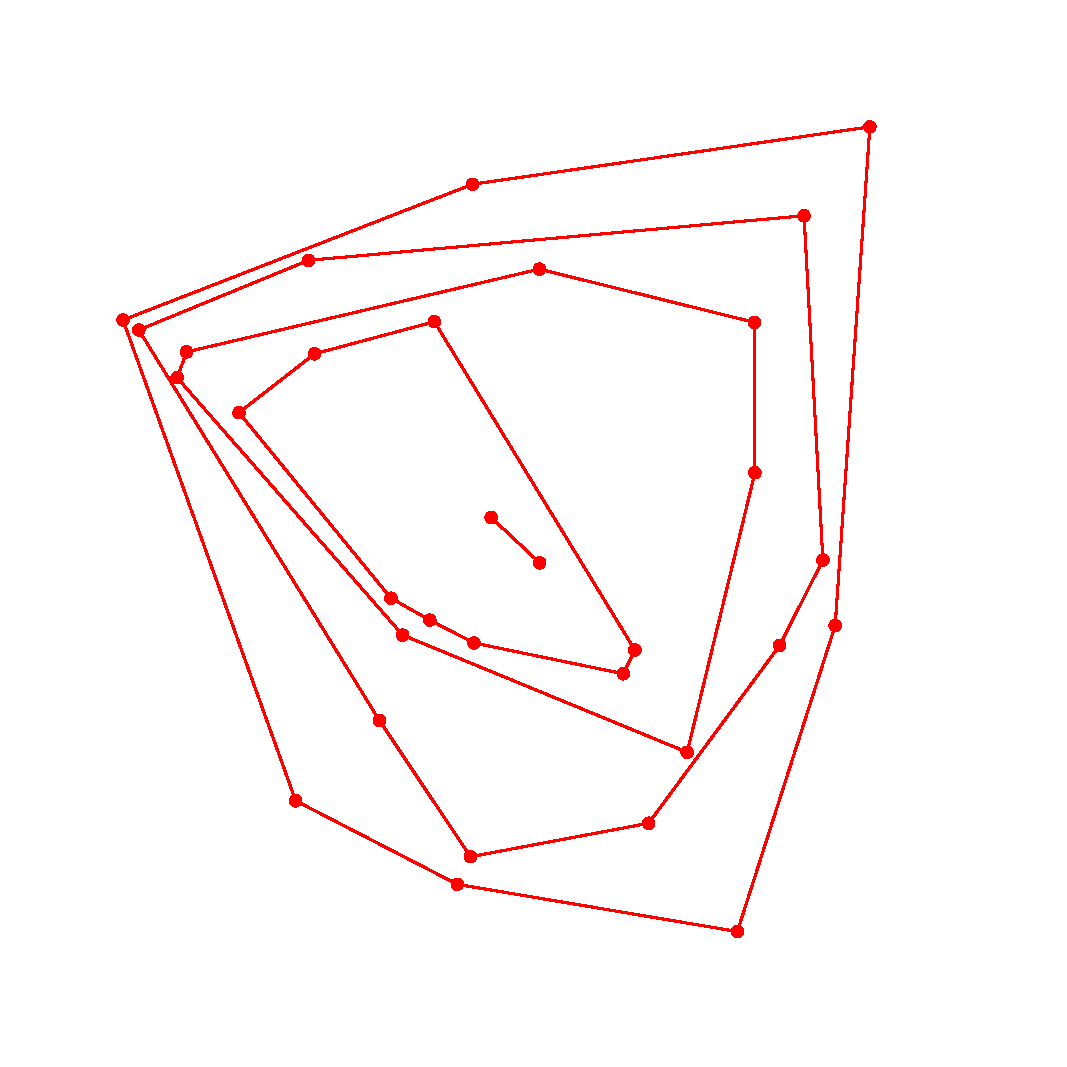
\includegraphics[width=0.45\textwidth]{Fig-FullConvexLayers} % {Fig-FullCHPeeling.pdf}
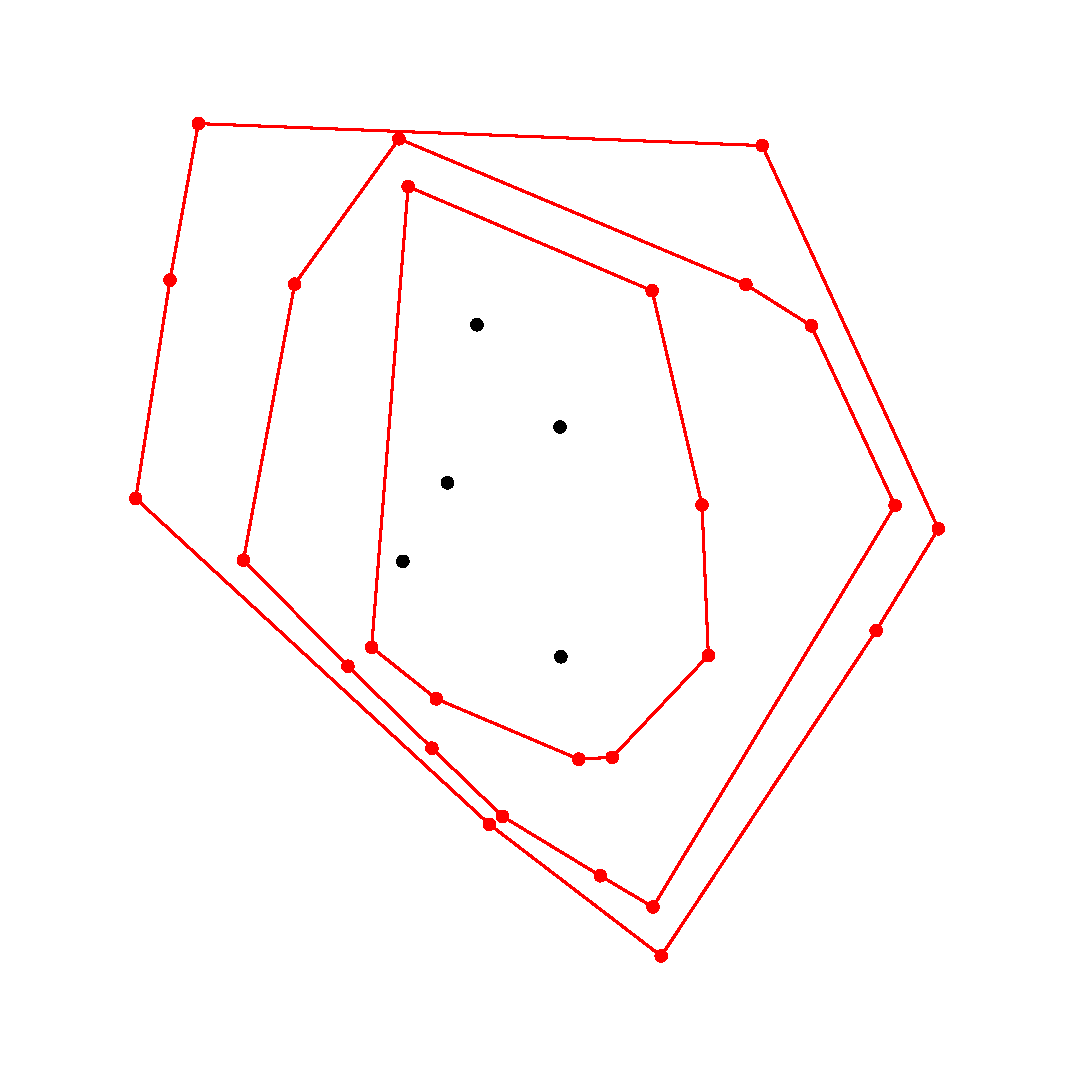
\includegraphics[width=0.45\textwidth]{Fig-PartialConvexLayers} %{Fig-PartialCHPeeling.pdf}
\caption{Full onion peeling with last layer indicating the convex depth (left) and partial onion peeling of the first $k=3$ layers.}
\label{fig:chpeeling}

\end{figure}

\end{itemize}

%\cite{DFSNeuromanifold-1991}

\bibliographystyle{plain}
%\bibliographystyle{annotate}
\bibliography{FrankNielsenPapersBIB}
\end{document}